\section{1174008 - Arjun Yuda Firwanda}

\subsection{Teori}
\begin{enumerate}

        \item Jelaskan dengan ilustrasi gambar sendiri apa itu generator dengan perumpamaan anda sebagai mahasiswa sebagai generatornya.

Generator merupakan generator yang biasanya menggunakan data yang ada untuk menghasilkan data baru, serta genarator sendiri bertujuan untuk menghasilkan data berupa video,gambar,audio dan teks.

	\begin{figure}[H]
            	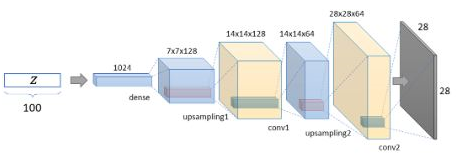
\includegraphics[width=4cm]{figures/1174008/8/teori1.PNG}
           	 \centering
           	 \caption{Generator}
        	\end{figure}

        \item Jelaskan dengan ilustrasi gambar sendiri apa itu diskriminator dengan Dosen sebagai Diskriminator.

Diskriminator merupakan untuk membedakan antara data nyata dan data yang dihasilkan oleh generator. pada jaringan diskriminator sendiri mencoba memasukan data ke dalamm kategori yang sudah ditentukan.

	\begin{figure}[H]
		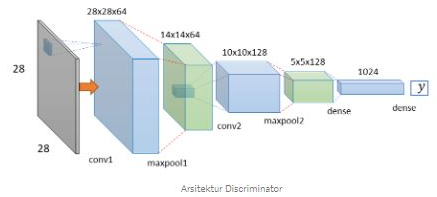
\includegraphics[width=4cm]{figures/1174008/8/teori2.PNG}
            	\centering
           	 \caption{Diskriminator}
       	 \end{figure}

        \item Jelaskan dengan ilustrasi gambar sendiri bagaimana arsitektur generator dibuat

Dilihat berkebalikan dengan struktur jaringan saraf pada umumnya. Pada Generator dinyatakan menerima input vektor z dan kemdian mengubahnya menjadi gambar tiga dimensi.

	\begin{figure}[H]
		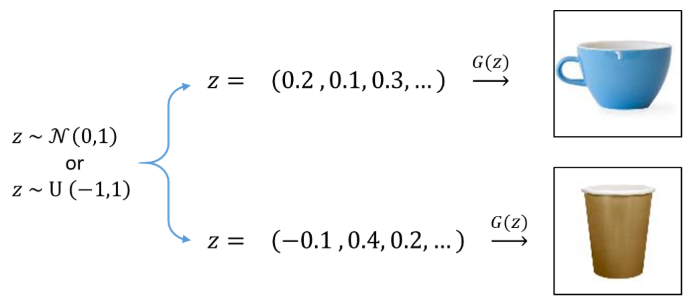
\includegraphics[width=4cm]{figures/1174008/8/teori3.PNG}
            	\centering
           	 \caption{Arsitektuk Generator}
       	 \end{figure}

        \item Jelaskan dengan ilustrasi gambar sendiri bagaimana arsitektur diskriminator dibuat

Diskriminator merupakan jaringan klasifikasi biner yang menerima input gambar tiga dimensi dan mengeluarkan klasifikasi gambar asli. Diskriminator dilatih dengan sekumpulan data, dan sekumpulan dataset, dan dilatih untuk bisa membedakan keduanya.

	\begin{figure}[H]
		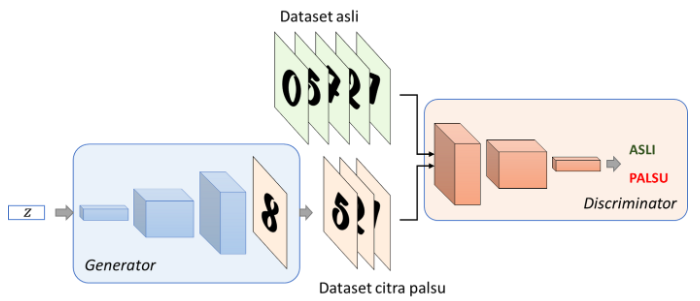
\includegraphics[width=4cm]{figures/1174008/8/teori4.PNG}
            	\centering
           	 \caption{Arsitektur Diskriminator}
       	 \end{figure}


        \item Jelaskan dengan ilustrasi gambar apa itu latent space.

Latent space merupakan vektor angka yang dihasilkan secara acak.

	\begin{figure}[H]
		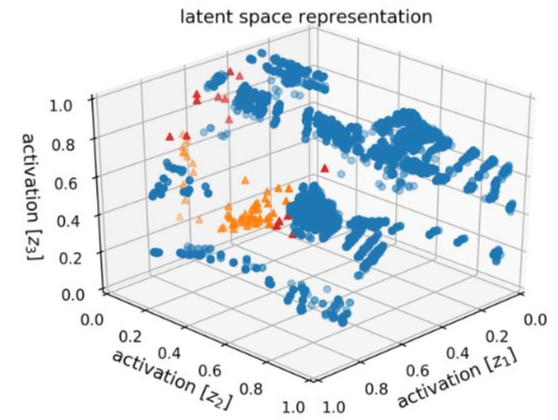
\includegraphics[width=4cm]{figures/1174008/8/teori5.PNG}
            	\centering
           	 \caption{Arsitektur Diskriminator}
       	 \end{figure}


        \item Jelaskan dengan ilustrasi gambar apa itu adversarial play

Advesarial Play, berbagi data pelestarian privasi, dan vaksin rancangan. Saya menjelaskan bagaimana aspek konseptual kedua dari game keamanan menawarkan pemodelan alami paradigma untuk ini.

	\begin{figure}[H]
		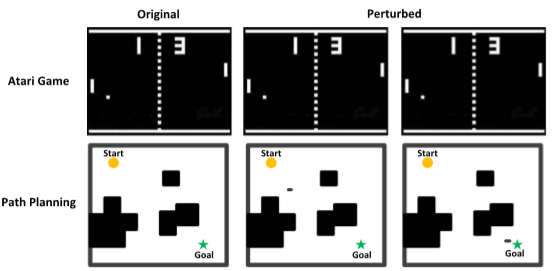
\includegraphics[width=4cm]{figures/1174008/8/teori6.PNG}
            	\centering
           	 \caption{Advesarial Play}
       	 \end{figure}

        \item Jelaskan dengan ilustrasi gambar apa itu Nash equilibrium

Nash Equilibrium sendiri menggambarkan keadaan tertentu dalam teori permainannya. Sehingga dalam permainan non kooperatif ini dimana setiap pemainnya memilihi strategi untuk hasil yang terbaik berdasarkan apa yang mereka harapkan apa yang dilakukan oleh pemain lainnya.

	\begin{figure}[H]
		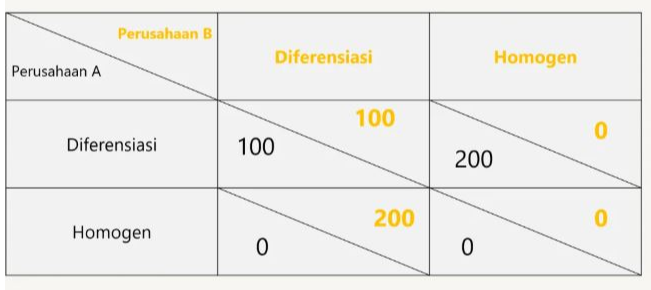
\includegraphics[width=4cm]{figures/1174008/8/teori7.PNG}
            	\centering
           	 \caption{Nash equilibrium}
       	 \end{figure}

        \item Sebutkan dan jelaskan contoh-contoh implementasi dari GAN

Cara membuat GAN dengan citra beresolusi tinggi. Kita mulai dengan data sederhana yang jauh lebih mudah, yaitu dataset citra angka tulisan tangan MNIST. Membangun GAN dengan library Keras dan Tensorflow. 

	\begin{figure}[H]
		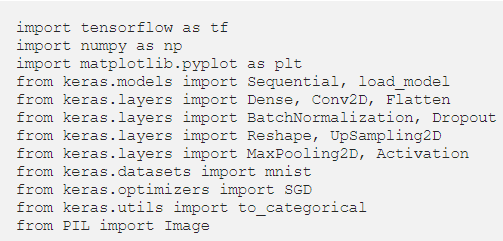
\includegraphics[width=4cm]{figures/1174008/8/teori8.PNG}
            	\centering
           	 \caption{GAN}
       	 \end{figure}

        \item Berikan contoh dengan penjelasan kode program beserta gambar arsitektur untuk membuat generator neural network dengan sebuah input layer, tiga hidden layer dense layer, dan satu output layer reshape layer

Inputan seed 1x100. Generator akan mengubah menjadi sebuah gambar 28x28  yang menggunakan Convolutional Neural Network.

	\begin{figure}[H]
		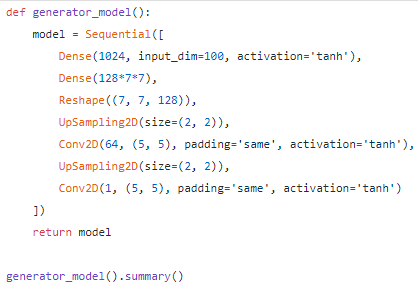
\includegraphics[width=4cm]{figures/1174008/8/teori9.PNG}
            	\centering
           	 \caption{Hasil Arsitektuk Generator}
       	 \end{figure}

        \item Berikan contoh dengan ilustrasi dari arsitektur dikriminator dengan sebuath input layer, 3 buah hidden layer, dan satu output layer.

Diskriminator merupakan CNN yang menerima input 28,28 dan menghasilkan angka biner, jika kelas 1 maka gambar asli, jika kelas 0 maka gambar palsu.

	\begin{figure}[H]
		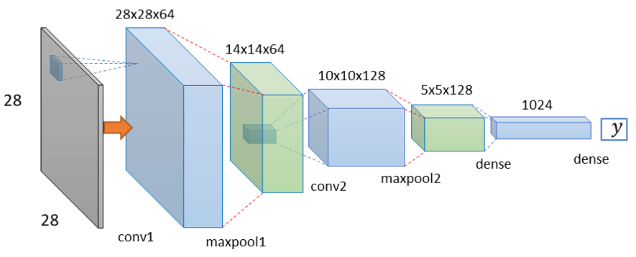
\includegraphics[width=4cm]{figures/1174008/8/teori10.PNG}
            	\centering
           	 \caption{Hasil Arsitektur Generator}
       	 \end{figure}

        \item Jelaskan bagaimana kaitan output dan input antara generator dan diskriminator tersebut. Jelaskan kenapa inputan dan outputan seperti itu.

Generator, Di sini kami tetapkan ukuran input seed adalah 1x100. Diskriminator, yang menerima input 28,28 dan menghasilkan angka biner, jika kelas 1 maka gambar asli, jika kelas 0 maka gambar palsu.

        \item Jelaskan apa perbedaan antara KullbackLeibler divergence KL divergence relative entropy, Jensen-Shannon JS divergence  information radius iRaD total divergence to the average dalam mengukur kualitas dari model.

Kullback-Leibler divergence untuk menghitung skor yang mengukur divergensi satu distribusi probabilitas dari yang lain. Jensen-Shannon divergence metode untuk mengukur kesamaan antara dua distribusi probabilitas. Ia juga dikenal sebagai radius informasi IRad atau total divergensi ke rata-rata.

        \item Jelaskan apa itu fungsi objektif yang berfungsi untuk mengukur kesamaan antara gambar yang dibuat dengan yang asli.

Fungsi obyektif digunakan untuk membuat jaringan gerator yang menghasilkan gambar yang mirip dengan 
gambar yang asli nya, serta meningkatkan kesamaan data yang dihasilkan oleh generator ke data aslinya.

	\begin{figure}[H]
		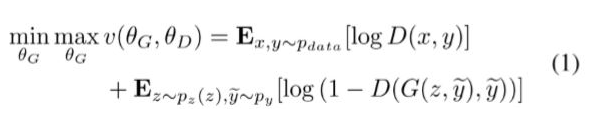
\includegraphics[width=4cm]{figures/1174008/8/teori13.PNG}
            	\centering
           	 \caption{Hasil Arsitektuk Generator}
       	 \end{figure}

        \item Jelaskan apa itu scoring algoritma selain mean square error atau cross entropy seperti The Inception Score dan The Frechet Inception distance.

The Inception Score memperkirakan kualitas koleksi gambar sintetis berdasarkan seberapa baik model klasifikasi gambar berkinerja terbaik Inception v3 mengklasifikasikannya sebagai salah satu dari 1.000 objek yang dikenal. Skor menggabungkan kepercayaan prediksi kelas bersyarat untuk setiap gambar sintetis kualitas dan integral dari probabilitas marginal dari kelas prediksi keragaman. The Frechet Inception Distance meringkas jarak antara vektor fitur Inception untuk gambar nyata dan yang dihasilkan dalam domain yang sama.

        \item Jelaskan kelebihan dan kekurangan GAN

Kelebihan GAN yang pertama dapat dijadikan sebagai pembelajaran tanpa pengawasan, kemudian yang kedua gan menghasilkan data yang mirip dengan aslinya, dan selanjutnya yang ketiga sebagai belajar distribusi kepadatan data.

Kekurangannya sulit dilatih, tidak stabil, serta terdapat masalah pada mode tutup.

\end{enumerate}

\subsection{Praktek}
\begin{enumerate}

	\item Jelaskan apa itu 3D convolutions
Konvolusi 3D menerapkan filter 3 dimensi ke dataset dan filter bergerak 3 arah x y z untuk menghitung representasi fitur level rendah. Bentuk output mereka adalah ruang volume 3 dimensi seperti kubus.

	\item Jelaskan dengan kode program arsitektur dari generator networknya, beserta penjelasan input dan output dari generator network.
Pada kode program ini, menyebutkan seed atau ketetapan ukuran input. Yakni 1x100 dan mengubahkan outputnya menjadi 28x28 yang menggunakan Convolution Neural Network.

		\lstinputlisting[firstline=1, lastline=40]{src/1174008/8/praktik2.py}

	\item Jelaskan dengan kode program arsitektur dari diskriminator network, beserta penjelasan input dan outputnya.
Pada program ini, input gambar berupa 28x28 dan menghasilkan angka biner yang menyatakan bahwa kelas 1 merupakan data asli, dan jila kelas 0 maka gambar palsu.

		\lstinputlisting[firstline=1, lastline=31]{src/1174008/8/praktik3.py}

	\item Jelaskan proses training 3D-GANs
Proses Training disini melatih data gambar menggunakan Generator
Bangkitkan data citra palsu menggunakan Generator sejumlah dataset citra asli.
Latih Discriminator untuk bisa membedakan dataset citra asli dari dataset citra palsu.
Gunakan Discriminator yang sudah dilatih untuk melatih Generator agar bisa membangkitkan dataset citra palsu yang dinilai asli oleh Discriminator.

        	\item Jelaskan bagaimana melakukan settingan awal chapter 02 untuk memenuhi semua kebutuhan sebelum melanjutkan ke tahapan persiapan data.
load dataset file csv.
menghasilkan label biner lulus gagal berdasarkan G1 G2 G3 nilai tes, masing-masing 0 20 poin ambang batas untuk kelulusan adalah jumlah 30.
gunakan one-hot encodin pada kolom kategorikal.
gunakan shuffle row.
menggunakan decision tree.
menggunakan visualisasi pohon.

        	\item Jelaskan tentang dataset yang digunakan, dari mulai tempat unduh, cara membuka dan melihat data. Sampai deskripsi dari isi dataset dengan detail penjelasan setiap folder yang membuat orang awam paham.
Isi dari dataset 3DShapeNets ada 6 folder. Dan masing-masing folder terdapat isi yang berbeda.
Folder 3D untuk gambar 3D
Folder bp untuk mendeskripsikan dan meneruskan program.
Folder generative untuk mengenerate data gambar.
Folder util untuk input json.
Folder volumetric data untuk mengetahui metrik volume data.
Folder voxelization untuk menampilkan hasil gambar berupa plot.

        	\item Jelaskan apa itu voxel dengan ilustrasi dan bahasa paling awam
Voxel diibaratkan seperti pixel di bidang tiga dimensi, memiliki panjang, lebar dan tinggi. Volume pixel atau voxel adalah titik dalam ruang tiga dimensi. Sebuah voxel mendefinisikan posisi dengan tiga koordinat dalam arah x, y, dan z. Sebuah voxel adalah unit dasar untuk mewakili gambar 3D

        	\item Visualisasikan dataset tersebut dalam tampilan visual plot, jelaskan cara melakukan visualisasinya
import library, load data file .mat, lalu read memakai matplotlib.

        	\item buka file run.py jelaskan perbaris kode pada fungsi untuk membuat generator yaitu build generator.
Membuat generator yaitu dengan ketentukan gen sebagai variabel dan membuat fungsi atau variabel gen model lalu dilakukan return

        	\item jelaskan juga fungsi untuk membangun diskriminator pada fungsi build discriminator.
Membangun diskriminator berfungsi untuk mendefenisikan seluruh gambar yang sudah di load generator sebagai gambar fake dan real

        	\item  jelaskan apa maksud dari kode program name  main
itu menetapkan beberapa variabel khusus seperti  name
itu mengeksekusi semua kode yang ditemukan dalam file.
Jika interpreter python menjalankan if name main  sebagai program utama, itu ialah menetapkan variabel name  untuk memiliki nilai main. Jika file ini sedang diimpor dari modul lain, name akan ditetapkan ke nama modul. Nama modul tersedia sebagai nilai untuk name variabel global.

		\lstinputlisting[firstline=1, lastline=1]{src/1174008/8/praktik11.py}

		\begin{figure}[H]
			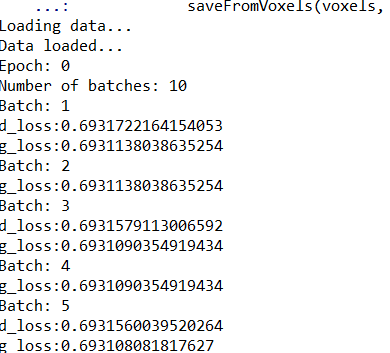
\includegraphics[width=4cm]{figures/1174008/8/praktik11.PNG}
            		\centering
           		\caption{File}
       	 	\end{figure}

        	\item jelaskan secara detil perbaris dan per parameter apa arti dari kode program :
Artinya adalah load dataset yang hanya dalam folder chair data train

		\lstinputlisting[firstline=1, lastline=13]{src/1174008/8/praktik12.py}

		\begin{figure}[H]
			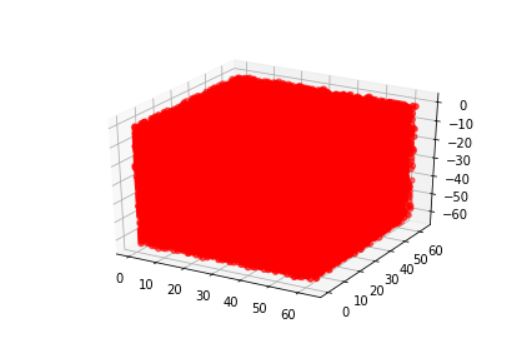
\includegraphics[width=4cm]{figures/1174008/8/praktik12.PNG}
            		\centering
           		\caption{Parameter}
       	 	\end{figure}

        	\item Jelaskan secara detil dari kode program pembuatan dan kompilasi arsitektur berikut 
Disini menggunakan Adam sebagai algoritma pengoptimalan dan binary crossentropy sebagai kerugian loss. 

		\lstinputlisting[firstline=1, lastline=11]{src/1174008/8/praktik13.py}

		\begin{figure}[H]
			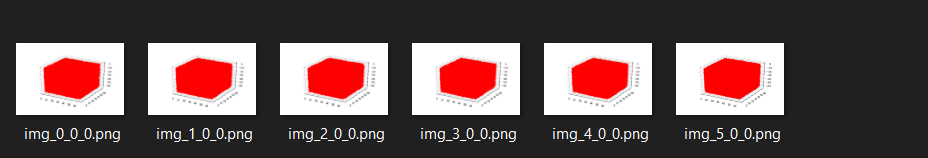
\includegraphics[width=4cm]{figures/1174008/8/praktik13.PNG}
            		\centering
           		\caption{Kompilasi Arsitektur}
       	 	\end{figure}

        	\item Jelaskan secara detil kode program untuk membuat dan melakukan kompilasi model adversarial berikut
Ini artinya ialah kita memasukkan random vector kedalam generator model lalu membagi 2 yaitu generated example dan real example, dan meneruskan ke diskriminator model sebagai real atau fake.

		\lstinputlisting[firstline=1, lastline=5]{src/1174008/8/praktik14.py}

		\begin{figure}[H]
			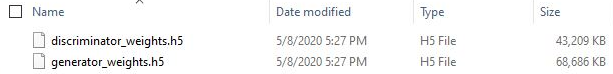
\includegraphics[width=4cm]{figures/1174008/8/praktik14.PNG}
            		\centering
           		\caption{Kompilasi Model Adversarial}
       	 	\end{figure}

        	\item Jelaskan Ekstrak dan load data kursi dengan menggunakan fungsi getVoxelsFormat dan get3DImages yang digunakan pada kode program berikut :
Ini melakukan load data pada dataset.

		\lstinputlisting[firstline=1, lastline=4]{src/1174008/8/praktik15.py}

        	\item Jelaskan maksud dari kode program instansiasi TensorBoard yang menambahkan generator dan diskriminator pada program berikut: 
Ini berfungsi untuk membuat tensorboard yang nantinya bisa diakses melalui localhost

		\lstinputlisting[firstline=1, lastline=3]{src/1174008/8/praktik16.py}

        	\item Jelaskan apa fungsi dari np reshape ones zeros pada kode program berikut dengan parameternya:
Fungsi ini ialah untuk melakukan reshape agar shape yang dihasilkan tidak terlalu besar.

		\lstinputlisting[firstline=1, lastline=2]{src/1174008/8/praktik17.py}

       	\item Jelaskan kenapa harus ada perulangan dalam meraih epoch. Dan jelaskan apa itu epoch terkait kode program berikut:
Karena jika epoch semakin banyak maka kualiatas training yang dihasilkan akan semakin baik

		\lstinputlisting[firstline=1, lastline=6]{src/1174008/8/praktik18.py}

        	\item Jelaskan apa itu batches dan kaitannya dengan kode program berikut, dan kenapa berada di dalam epoch:
Batch adalah jumlah file yang akan di training

		\lstinputlisting[firstline=1, lastline=4]{src/1174008/8/praktik19.py}

        	\item Berikut adalah kode program pengambilan gambar dan noise. Jelaskan apa fungsi np.random.normal serta astype, serta jelaskan apa arti parameter titik dua dan jelaskan isi dari z sample dan volumes batch:
Ini adalah untuk membuat gambar bersih dari noise dan juga menyesuaikan shape

		\lstinputlisting[firstline=1, lastline=2]{src/1174008/8/praktik20.py}

        	\item Berikut adalah kode program generator gambar palsu. Jelaskan apa fungsi generator.predict on batch, serta jelaskan apa arti parameter z sample:
Ialah membuat sample gambar palsu yang akan diteruskan ke diskriminator.

		\lstinputlisting[firstline=1, lastline=2]{src/1174008/8/praktik21.py}

        	\item Berikut adalah kode program training diskriminator dengan gambar palsu dari generator dan gambar asil. Jelaskan apa maksudnya harus dilakukan training diskriminator secara demikian dan jelaskan apa isi loss fake dan loss real serta d loss dan fungsi train on batch.
Diskriminator bisa load gambar fake dan real dari generator, oleh karena itu ada generator loss dan diskriminator loss untuk melihat seberapa baik kualitas yang dihasilkan.

		\lstinputlisting[firstline=1, lastline=13]{src/1174008/8/praktik22.py}

        	\item Berikut adalah kode program training model adversarial yang terdapat generator dan diskriminator. Jelaskan apa bagaimana proses terbentuknya parameter z dan g loss:
Dengan melakukan print g loss untuk generator dan juga d loss untuk diskriminator

		\lstinputlisting[firstline=1, lastline=6]{src/1174008/8/praktik23.py}

        	\item Berikut adalah kode program generate dan menyimpan gambar 3D setelah beberapa saat setiap epoch. Jelaskan mengapa ada perulangan dengan parameter tersebut, serta jelaskan arti setiap variabel beserta perlihatkan isinya dan artikan isinya:
Mengapa ada perulangan ? karena untuk melakukan perbandingan dari hasil yang sudah didapat.

		\lstinputlisting[firstline=1, lastline=10]{src/1174008/8/praktik24.py}

        	\item Berikut adalah kode program menyimpan average losses setiap epoch. Jelaskan apa itu tensorboard dan setiap parameter yang digunakan pada kode program ini:
TensorBoard adalah sebuah aplikasi web localhost untuk memeriksa dan menyelesaikan grafik dari hasil TensorFlow.

		\lstinputlisting[firstline=1, lastline=3]{src/1174008/8/praktik25.py}

        	\item Berikut adalah kode program menyimpan model. Jelaskan apa itu format h5 dan penjelasan dari kode program berikut:
File H5 adalah file data yang disimpan dalam Format Data Hirarki. Ini berisi array multidimensi data ilmiah.

		\lstinputlisting[firstline=1, lastline=5]{src/1174008/8/praktik26.py}

        	\item Berikut adalah kode program testing model. Jelaskan dengan ilustrasi gambar dari mulai meload hingga membuat gambar 3D dengan menggunakan z sample, bisakah parameter z sample tersebut diubah2:
Ini adalah tahap akhir untuk melakukan testing dari model yang telah dibuat dan buat model dari yang sudah di create sebelumnya yaitu generator dan diskriminator.

		\lstinputlisting[firstline=1, lastline=18]{src/1174008/8/praktik27.py}

\end{enumerate}

\subsection{Penanganan Error}


\subsection{Bukti Tidak Plagiat}
\begin{figure}[H]
	\centering
	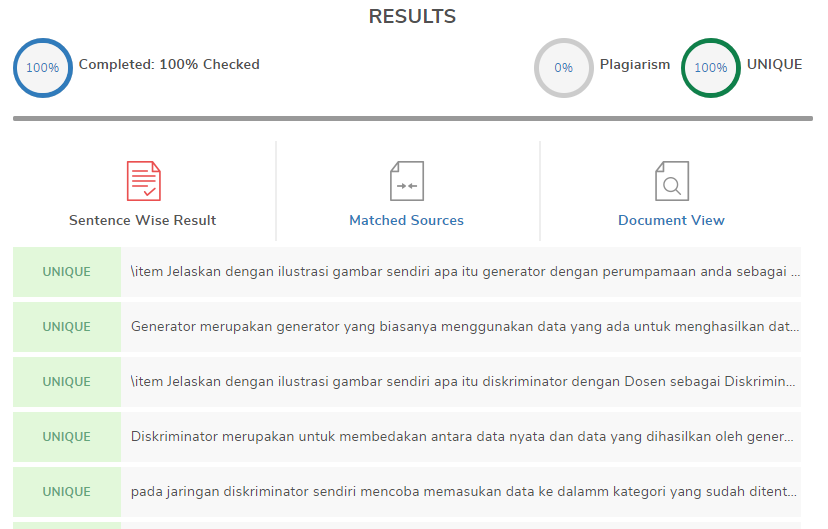
\includegraphics[width=4cm]{figures/1174008/8/bukticekplagiarismechapter8.PNG}
	\caption{Bukti Tidak Melakukan Plagiat Chapter 8}
\end{figure}